\documentclass{beamer}
\beamertemplatenavigationsymbolsempty
\usecolortheme{beaver}
\newcommand{\norm}[1]{\left\lVert#1\right\rVert}
\setbeamertemplate{blocks}[rounded=true, shadow=true]
\setbeamertemplate{footline}[page number]
%
\usepackage[utf8]{inputenc}
\usepackage[english,russian]{babel}
\usepackage{amssymb,amsfonts,amsmath,mathtext}
\usepackage{subfig}
\usepackage[all]{xy} % xy package for diagrams
\usepackage{array}
\usepackage{multicol}% many columns in slide
\usepackage{hyperref}% urls
\usepackage{hhline}%tables
% Your figures are here:
\graphicspath{ {fig/} {../paper/figures} }

%----------------------------------------------------------------------------------------------------------
\title[\hbox to 56mm{Восстанвление прогноза}]{Восстановление прогноза, сделанного в метрическом вероятностном пространстве, в исходное пространство (временных рядов)}
\author[М. М. Дивильковский]{Максим Михайлович Дивильковский}
\institute{Московский физико-технический институт}
\date{\footnotesize
	\par\smallskip\emph{Курс:} Автоматизация научных исследований\par (практика, В.\,В.~Стрижов)/Группа 125
	\par\smallskip\emph{Эксперт:} В. В. Стрижов
	\par\smallskip\emph{Консультант:} К. Д. Яковлев
	\par\bigskip\small 2024}
%----------------------------------------------------------------------------------------------------------
\begin{document}
%----------------------------------------------------------------------------------------------------------
\begin{frame}
\thispagestyle{empty}
\maketitle
\end{frame}
%-----------------------------------------------------------------------------------------------------
\begin{frame}{Цель исследования}
	Решается задача прогнозирования набора высококоррелированных рядов.
	
	\begin{columns}[c]
		\column{0.7\textwidth}
		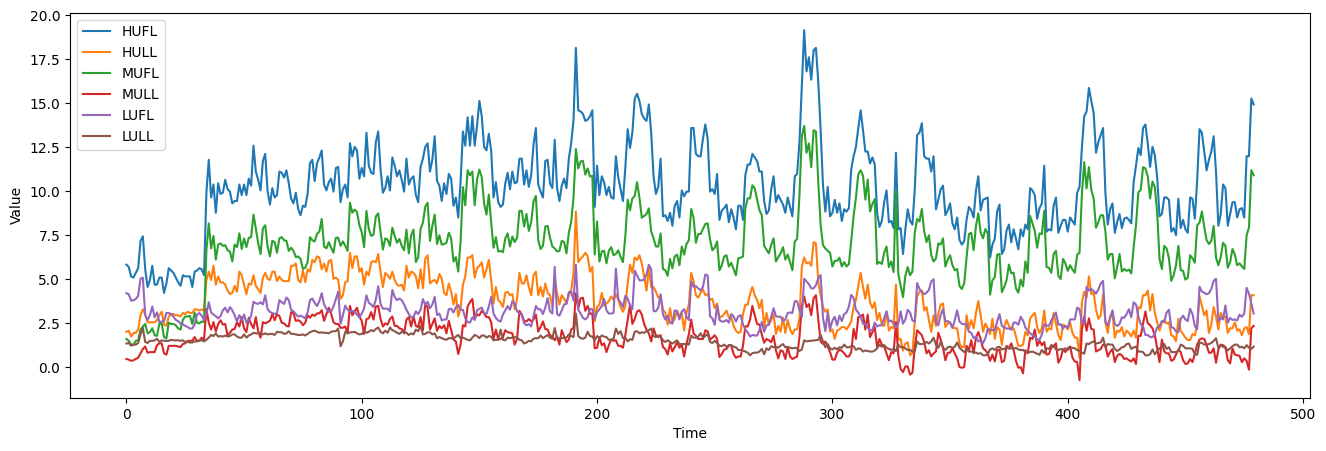
\includegraphics[width=1.0\textwidth]{Electricity}
		Набор данных ETTh1
		\column{0.3\textwidth}
		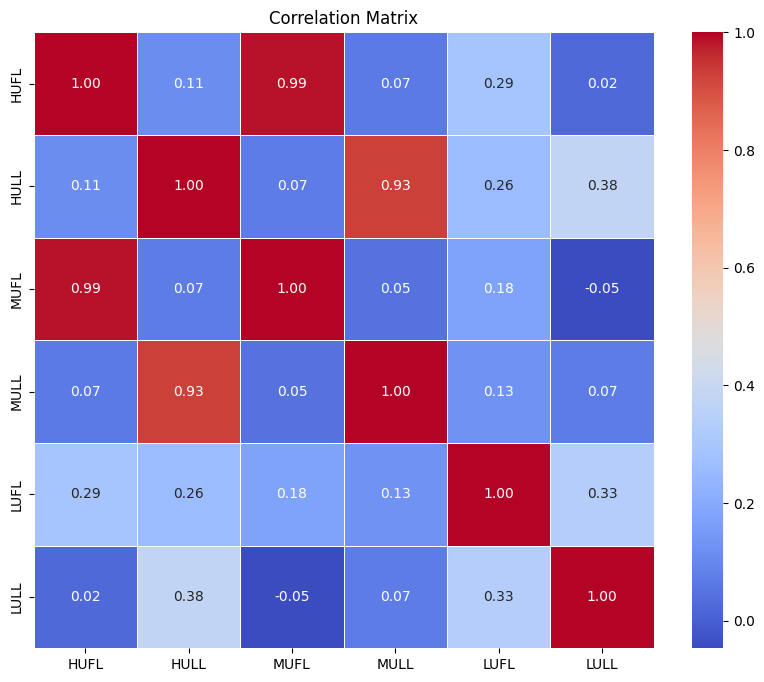
\includegraphics[width=1.0\textwidth]{Correlation}
		Попарная корреляция между рядами
	\end{columns}
\end{frame}
%-----------------------------------------------------------------------------------------------------
\begin{frame}{Цель исследования}

\begin{columns}[c]
	\column{0.5\textwidth}
	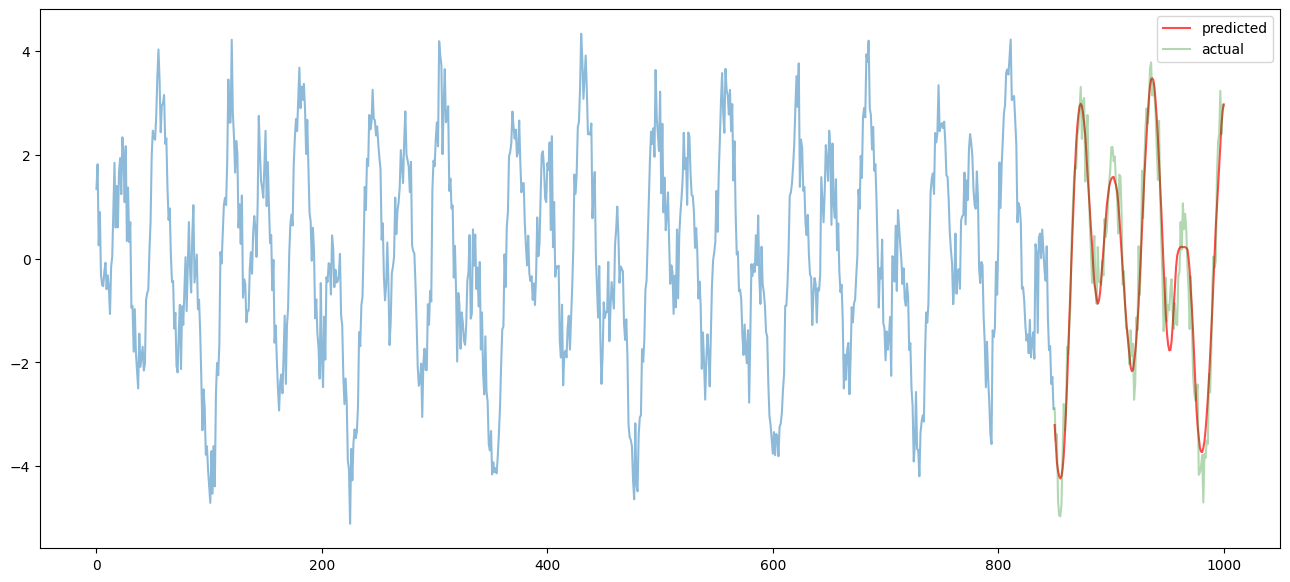
\includegraphics[width=1.0\textwidth]{LSTM-prediction}
	Предсказание методом LSTM
	\column{0.5\textwidth}
	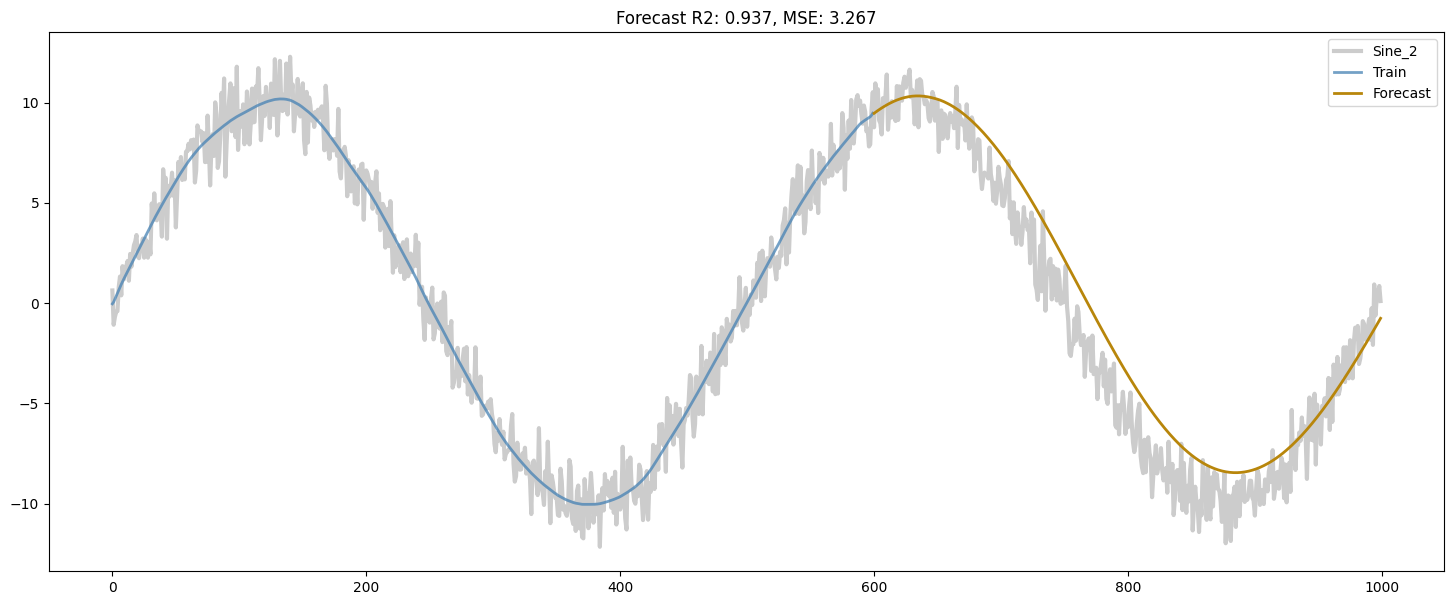
\includegraphics[width=1.0\textwidth]{MSSA-prediction}
	Предсказание методом MSSA
\end{columns}
\bigskip
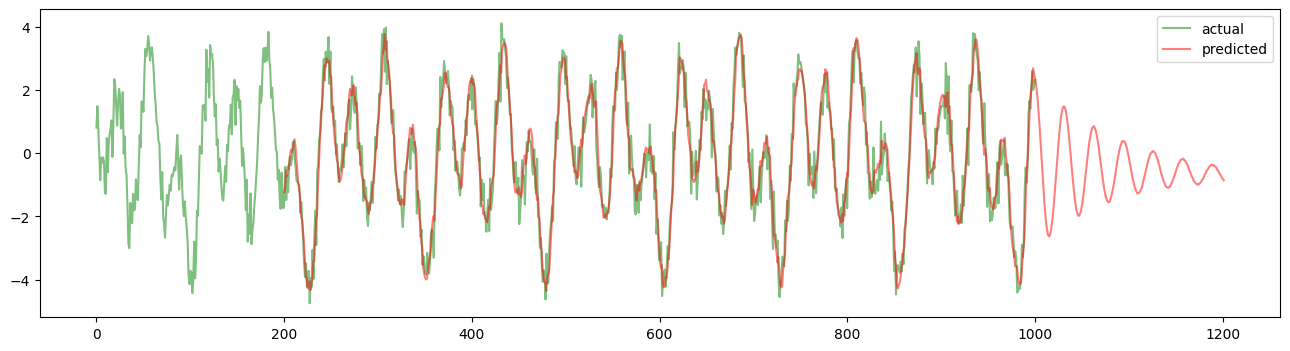
\includegraphics[width=1.0\textwidth]{SARIMA-prediction}
Предсказание методом SARIMA

\end{frame}


%----------------------------------------------------------------------------------------------------------
\begin{frame}{Источники}
	\begin{itemize}
		\item James B. Elsner and Anastasios A. Tsonis. Singular spectrum analysis: A new tool in time series analysis.
		1996.
		
		\item Sima Siami-Namini and Akbar Siami Namin. Forecasting economics and financial time series: Arima vs.
		lstm, 2018.
		
		\item Haoyi Zhou, Shanghang Zhang, Jieqi Peng, Shuai Zhang, Jianxin Li, Hui Xiong, and Wancai Zhang.
		
		Informer: Beyond efficient transformer for long sequence time-series forecasting, 2021.
		\item Ailing Zeng, Muxi Chen, Lei Zhang, and Qiang Xu. Are transformers effective for time series forecasting?,
		2022.
		
	\end{itemize}
\end{frame}

%----------------------------------------------------------------------------------------------------------
\begin{frame}{Постановка задачи}

\begin{itemize}
	\item $X$~--- линейное пространство временных рядов. $X \cong \mathbb{R}^{T}$
	\item $\rho(x, y), x, y \in X$~--- расстояния в $X$
	\item $X \rightarrow \Sigma_T$~--- матрица попарных расстояний
	\item $\Sigma_T \rightarrow \Sigma_{T+1}$~--- прогноз в следующий момент времени
	\item $\Sigma_{T+1} \rightarrow \hat{X}$~--- {\color{red}восстановление прогноза}
	
\end{itemize}
\end{frame}
%----------------------------------------------------------------------------------------------------------
\begin{frame}{Постановка задачи восстановления прогноза}
	$$\Sigma_{t+1} = \left(
	\begin{array}{cccc}
		d(\mathbf{x}^{(1)}, \mathbf{x}^{(1)}) & d(\mathbf{x}^{(1)}, \mathbf{x}^{(2)}) & \ldots & d(\mathbf{x}^{(1)}, \mathbf{x}^{(n)})\\
		d(\mathbf{x}^{(2)}, \mathbf{x}^{(1)}) & d(\mathbf{x}^{(2)}, \mathbf{x}^{(2)}) & \ldots & d(\mathbf{x}^{(2)}, \mathbf{x}^{(n)})\\
		\vdots & \vdots & \ddots & \vdots\\
		d(\mathbf{x}^{(n)}, \mathbf{x}^{(1)}) & d(\mathbf{x}^{(n)}, \mathbf{x}^{(2)}) & \ldots & d(\mathbf{x}^{(n)}, \mathbf{x}^{(n)})\\
	\end{array}
	\right)$$
	
	Функция $d$~--- некоторая функция расстояния между рядами (корреляция, евклидово расстояние и т.д.).
	
	$\bigskip$
	
	Решается задача $\underset{y}{\mathrm{argmin}} \norm{\Sigma_{t+1} - \hat{\Sigma}_{t+1}}_2^2$
\end{frame}
\begin{frame}{Примеры метрик}
	\begin{columns}[c]
		\column{0.45\textwidth}
		\textbf{Евклидово расстояние}
		$$d(p,q)=\sqrt{\sum_{k=1}^n (p_k-q_k)^2}$$
		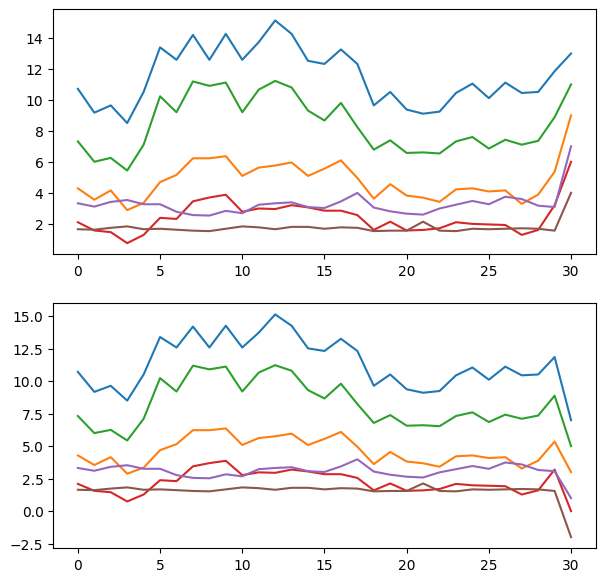
\includegraphics[width=1.0\textwidth]{EuclideanMetric}
		
		\column{0.55\textwidth}
		\textbf{Корреляция}
		$$
			\hat{\Sigma}_T = \frac{1}{T} \sum_{t=1}^{T} (x_t - \mu_T)(x_t - \mu_T)^T
		$$
		$$
			\mu_T = \frac{1}{T} \sum_{t=1}^{T} x_t
		$$
		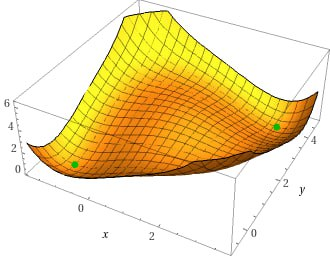
\includegraphics[width=0.7\textwidth]{CorrelationError}
		
		Решения задачи для рядов (1 3) и (2 4)~--- точки (3; 4) и $\textbf{(-1, 0)}$
	\end{columns}
\end{frame}

\begin{frame}{Теоретическая часть}
	\textbf{Теорема 1.} \textit{Для любой метрики, введённой в пространстве временных рядов $\mathbb{R}^t$, существует более одного способа восстановить исходные временные ряды по построенной матрице попарных расстояний.}
	
	\textbf{Доказательство.} 
	\begin{itemize}
		\item Метрика~--- непрерывная функция из $\mathbb{R}^t \times \mathbb{R}^t$ в $\mathbb{R}$.
		$d(x_n,y_n)\leqslant d(x_n,x)+d(x,y)+d(y_n,y)\to d(x,y)$
		
		\item Не существует гомеоморфизма между $\mathbb{R}^t \times \mathbb{R}^t$ и $\mathbb{R}$.
		
		\item Метрика~--- строго \textbf{сюръекция}.
	\end{itemize}
	
	\textbf{Следствие из доказательства.} \textit{Данное утверждение выполняется для произвольной непрерывной функции, в том числе попарной корреляции.}
\end{frame}
%----------------------------------------------------------------------------------------------------------
\begin{frame}{Попарная корреляция}
	\begin{gather*}
		\hat{\Sigma}_T = \frac{1}{T} \sum_{t=1}^{T} (x_t - \mu_T)(x_t - \mu_T)^T\\
		\mu_T = \frac{1}{T} \sum_{t=1}^{T} x_t
	\end{gather*}
	\textbf{Теорема 2.} \textit{В случае, если мы точно спрогнозировали матрицу расстояний, функция} $||\hat{\Sigma}_{t+1} - \bar{\Sigma}_{t+1}||_2^2$ \textit{будет иметь два минимума, задающихся следующим образом:}
	\begin{align*}
		\hat{y_i} &= y_i\\
		\hat{y_i} &= \frac{2}{T-1} \sum_{k=1}^{T-1} a_{ik} - y_i,
	\end{align*}
	\textit{где} $\hat{y}_i$~--- $i$\textit{-я координата предсказываемого значения ряда в момент $T+1$, $A=(a_{ik})$~--- исходный многомерных временной ряд,} $y_i$~--- \textit{истинные значения ряда в момент} $T+1$.
	
\end{frame}
%----------------------------------------------------------------------------------------------------------
\begin{frame}{Явный вид минимума}
	\textbf{Теорема 3.} \textit{Минимум функции $||\hat{\Sigma}_{t+1} - \bar{\Sigma}_{t+1}||_2^2$ достигается на \[\pm\sqrt{\lambda_1} u_1 + \mu_T,\] где $\lambda_1$--- первое сингулярное значение, $u_1$--- первый левый сигнулярный вектор матрицы $A=\left(\frac{T}{T+1} \cdot \Sigma_T - \Sigma_{T+1}\right) \cdot \frac{(T+1)^2}{T}$}
	
	$\bigskip$

	Эта теорема позволяет находить оба минимума функции намного быстрее, чем при использовании стандартных методов оптимизации.
	
\end{frame}
%----------------------------------------------------------------------------------------------------------
\begin{frame}{Алгоритм прогноза}
	Предлагается следующий алгоритм:
	
	1. Зафиксируем $T$ и $T': T \neq T'$.
	
	2. Для $T$ и $T'$ произведем полученный выше алгоритм и получим наборы ответов: $[ans_1, ans_2], [ans'_1, ans'_2]$.
	
	3. Найдём тот ответ, который лежит в пересечении.
	\begin{figure}[H]
		\centering
		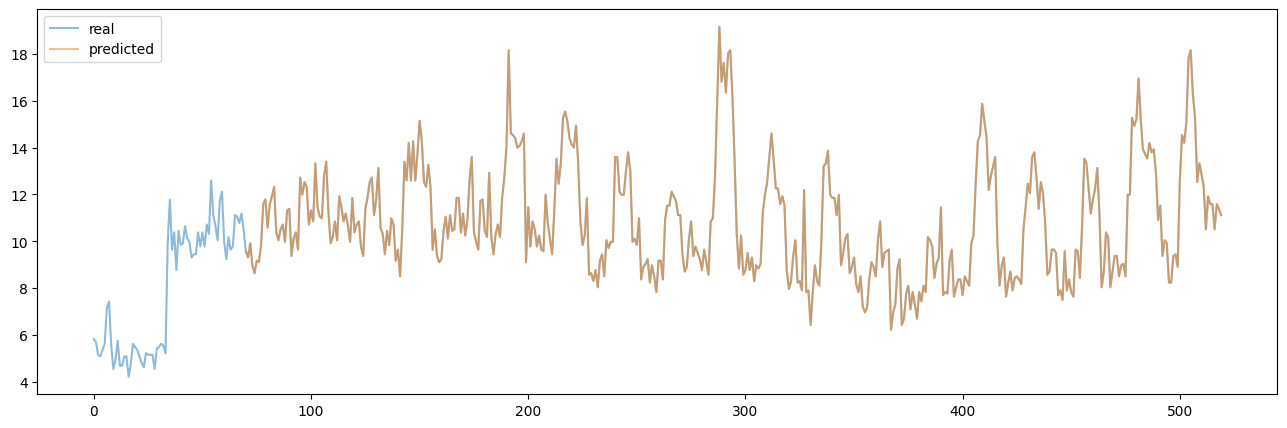
\includegraphics[width=\textwidth]{TwoTAlgo.png}
		\caption{Возвращение прогноза при идеальном прогнозе Sigma. $T=20$, $T'=10$}
		\label{fig:fig3}
	\end{figure}
\end{frame}
%----------------------------------------------------------------------------------------------------------
\begin{frame}{Алгоритм прогноза}
	\begin{figure}[H]
		\centering
		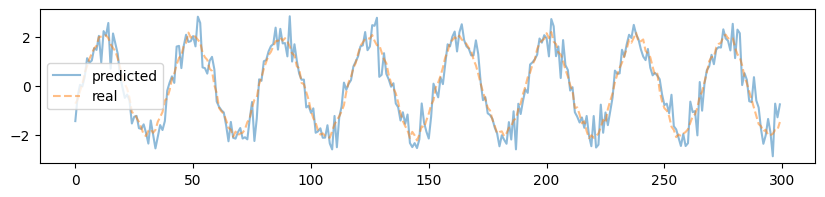
\includegraphics[width=\textwidth]{NonIdeal.png}
		\caption{Возвращение прогноза при неидеальном прогнозе Sigma $+ N(0, 0.1)$ с использованием двух матриц. MAE: 0.3662}
		\label{fig:fig4}
	\end{figure}
	\begin{figure}[H]
		\centering
		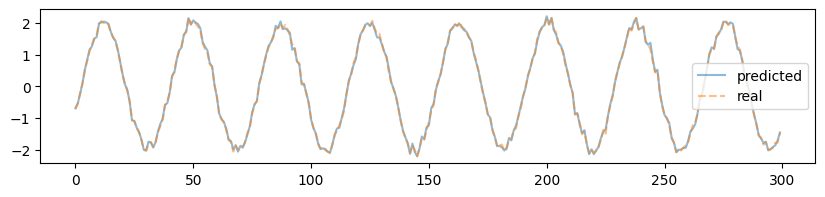
\includegraphics[width=\textwidth]{NonIdealBetter.png}
		\caption{Возвращение прогноза при неидеальном прогнозе Sigma $+ N(0, 0.01)$ с использованием трёх матриц. MAE: 0.03}
		\label{fig:fig5}
	\end{figure}
\end{frame}
%----------------------------------------------------------------------------------------------------------
\begin{frame}{Заключение}
    \begin{block}{Выводы}
    \begin{itemize}
        \item Показана невозможность использования метрического метода прогноза временных рядов.
        \item Показан явный вид минимума функции, минимизирующий ошибку.
        \item Предложен алгоритм восстановления при точном и неточном прогнозе.
    \end{itemize}
    \end{block}
    \begin{block}{Возможные пути развития}
    \begin{itemize}
    	\item Оценка диаметра ошибки
    \end{itemize}
    \end{block}
\end{frame}
%----------------------------------------------------------------------------------------------------------
\end{document} 